\documentclass[../diplomski_rad.tex]{subfiles}

\begin{document}

\sloppy

\justifying

\section{Bioimpedancija}

Bioimpedancija predstavlja električni otpor koji se javlja kada kroz biološka tkiva teče električna struja.
Ovisna je o frekvenciji te se može prikazati formulom:
\begin{equation}
    \label{jed:cpe}
    Z(f) = R_{e}(f) + jI_{m}(f) = |Z(f)|\angle\theta(f) 
\end{equation}
gdje je
\begin{equation}
    \label{jed:cpe}
    |Z(f)| = \sqrt{R_{e}^{2} + I_{m}^{2}}
\end{equation} 
\begin{equation}
    \label{jed:cpe}
    \theta(f) = arctg(\frac{I_{m}}{R_{e}})
\end{equation} 

\begin{figure}[htb]
    \centering
    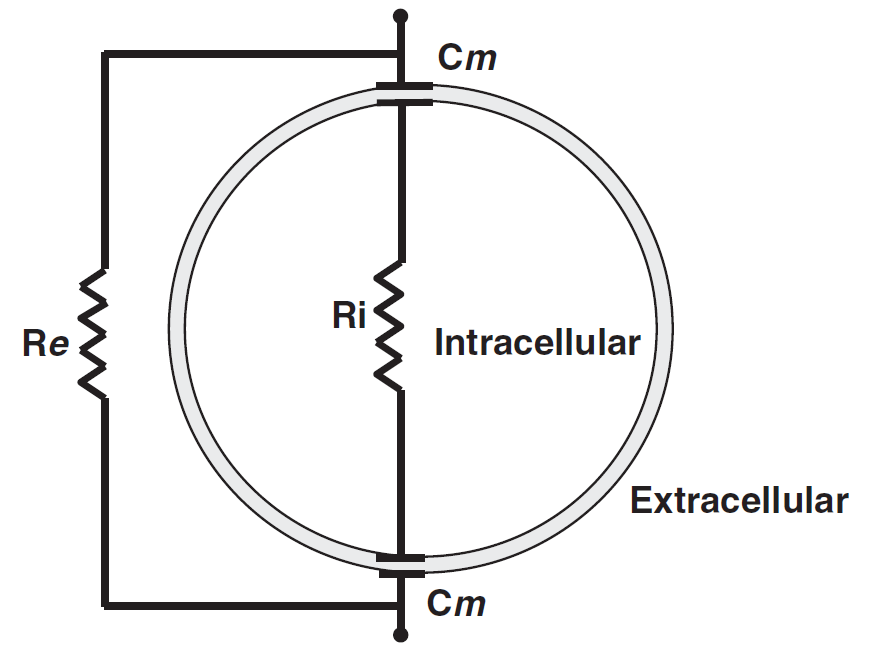
\includegraphics[width=0.6\textwidth]{Figures/stanica.png} 
    \caption{Električni model stanice \cite{Lukaski2013}}
    \label{slk:stanica}
\end{figure}
Za razumijevanje protoka električne struje kroz ljudsko tijelo, potrebno je detaljno prikazati električni model stanice.
Ljudska stanica može se modelirati ekvivalentnom električnom RC mrežom \cite{Lukaski2013}, 
kao što je prikazano na slici \ref{slk:stanica}. 
$R_{e}$ prestavlja otpor ekstracelularne tekučine dok $R_{i}$ prestavlja otpor intracelularne tekućine.
Stanična membrana zbog svojih kapacitivnih svojstava, prikazanih kapacitetom $C_{m}$, 
propušta struju visokih frekvencija, dok struje niskih frekvencija blokira. 
Zbog toga postoji razlika u mjerenoj impedanciji u ovisnosti o frekvenciji uzbudne struje. 
Na niskim frekvencijama struja samo vidi otpor $R_{e}$ ekstracelularne tekućine, dok se na visokim frekvencijama dodaje i otpor 
$R_{i}$ intracelularne tekućine čime ukupna impedancija pada.

-treba li dodavat ona 4 podrucja frekvencija ako se to kasnije nece koristit/spominjat?

Matematički model kojim se najčešće modelira bioimpedancija ljudskog tijela naziva se Cole model. 
Razvio ga je britanski fizičar Kenneth Cole 1940-tih godina. 
Cole model opisuje impedanciju tijela kao funkciju frekvencije zbog čega ga koristimo pri analizi sastava ljudskog tijela \cite{Freeborn2021}.
\begin{figure}[htb]
    \centering
    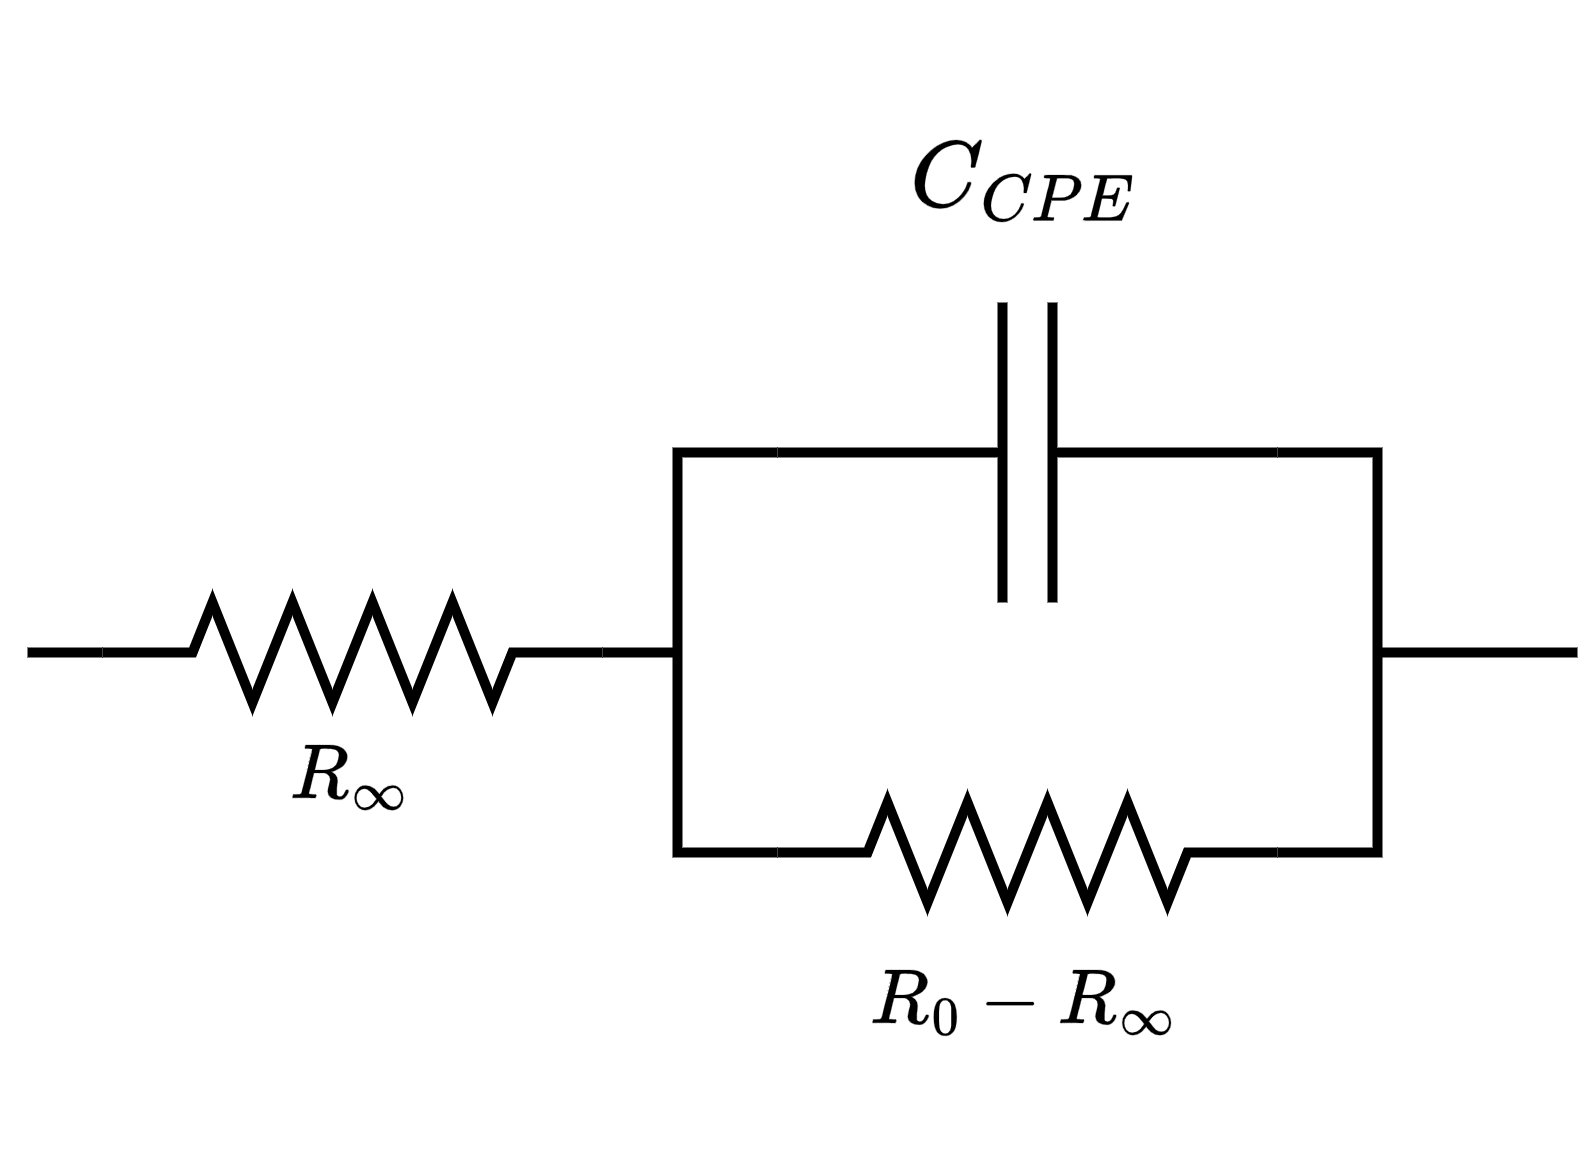
\includegraphics[width=0.6\textwidth]{Figures/cole_model.png} 
    \caption{Cole model bioimpedancije}
    \label{slk:cole_model}
\end{figure}
$R_{\infty}$ prestavlja otpor tkiva na beskonačnoj frekvenciji dok $R_{0}$ prestavlja otpor na nultoj frekvenciji. 
Razlika otpora $R_{0}-R_{\infty}$ predstavlja dodatan otpor struji na niskim frekvencijama zbog nepropusnosti stanične membrane. 
$C_{CPE}$ je element s konstantnom fazom koji modelira kapacitivnost stanične membrane 
te predstavlja neidealan kondenzator. Njegova impedancija iznosi: 
\begin{equation}
    \label{jed:cpe}
    Z_{CPE}(\omega) = \frac{1}{(j\omega)^{\alpha}C}
\end{equation} 
gdje je C kapacitet, a $\alpha$ njegov red. Kada je $\alpha = 0$ element s konstantnom fazom predstavlja idealan otpornik, 
dok sa $\alpha = 1$ predstavlja idealan kondenzator. 
Tipične vrijednosti parametra $\alpha$ za biološka tkiva su u intervalu 0.5 $< \alpha <$ 1 \cite{Freeborn2021}.
Ako uvedemo karakterističnu vremensku konstantu $\tau$ kao
\begin{equation}
    \label{jed:time_const}
    \tau = [(R_{0}-R_{\infty})C]^{1/\alpha}
\end{equation}
dobivamo orginalnu jednadžbu Cole modela: 
\begin{equation}
    \label{jed:cole}
    Z(\omega) = R_{\infty}+\frac{R_{0}-R_{\infty}}{1+(j\omega\tau)^{\alpha}} 
\end{equation} 
Iz jednadžbe \ref{jed:cole} vidljivo je kako su parametri Cole modela bioimpedancije 
$R_{\infty}$, $R_{0}$, $\alpha$ i $\tau$. 
Svojstva tkiva opisuju se pomoću navedenih parametra, a postupak kojim se do njih dolazi opisan je u daljnjem tekstu.

Rezultati mjerenja bioimpedancije na razilčitim frekvencijama mogu se aproksimirati polukružnicom,  
što je prikazano na slici \ref{slk:cole_graf}. 
Graf prikazuje omjer negativne reaktancije i otpora tkiva na svim frekvencijama, 
od $f=0$ do $f=\infty$. Frekvencija raste s desna na lijevo. 
\begin{figure}[htb]
    \centering
    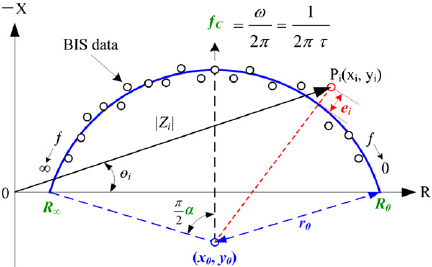
\includegraphics[width=0.7\textwidth]{Figures/cole_plot.png} 
    \caption{Graf bioimpedancije Cole modela \cite{Yang_2013}}
    \label{slk:cole_graf}
\end{figure}
Iz opisanog grafa moguće je dobiti parametre Cole modela \cite{Yang_2013}.
$R_{\infty}$ i $R_{0}$ jednostavno se iščitavaju kao presjecišta polukružnice i realne osi.
Vremenska konstanta $\tau$ inverz je karakteristične kružne frekvencije $\omega_{C}$ na kojoj je reaktancija najveća.
Relacija iz koje se izračunava $\tau$ je:
\begin{equation}
    \label{jed:cole}
    f_{C} = \frac{\omega_{C}}{2\pi} = \frac{1}{2\pi\tau} 
\end{equation} 
Parametar $\alpha$ određuje koliko je središte kružnice pomaknuto ispod realne osi. 
Izračunava se iz kuta između karakteristične frekvencije $f_{C}$ i beskonačne frekvencije $f_{\infty}$. 
Ako se taj kut definira kao $\theta$, vrijedi sljedeći izraz:
\begin{equation}
    \label{jed:cole}
    \theta = \frac{\pi}{2}\alpha 
\end{equation} 

\section{Pregled metoda mjerenja bioimpedancije}
Analiza bioimpedancije (engl. \textit{Bioelectrical Impedance Analysis; BIA}) klasificira se u dva pristupa: 
analiza s jednom frekvencijom (engl. \textit{Single frequency BIA; SF-BIA}) 
i analiza s višestrukim frekvencijama (engl. \textit{Multi frequency BIA; MF-BIA}).
Važna metoda je i bioelektrična spektrografija (engl. \textit{Bioelectrical spectroscopy; BIS}) 
koja daje rezultate kroz širok raspon frekvencija. 

SF-BIA je najjednostavnija i najbrža metoda jer koristi samo mjerenje impedancije na jednoj frekvenciji, najčešće 50 kHz. 
Iz izmjerene bioimpedancije matematičkim izračunima dobivaju se ukupna tjelesna voda, mišićna masa i masa masnog tkiva. 
Ova metoda ima najmanju preciznost jer se podatci prikupljaju na samo jednoj frekvenciji uzbudne struje.

MF-BIA koristi nekoliko različitih frekvencija čime se postiže veća točnost i mogućnost procjene dodatnih parametara, 
kao što su količine intracelularne i ekstracelularne vode. To je moguće jer stanična membrana blokira struju na niskim frekvencijama, 
a propušta ju na višim. 

Bioelektrička spektrografija najpreciznija je metoda mjerenja bioimpedancije. 
Mjerenja se vrše na širokom rasponu frekvencija, od 1 kHz do 1 MHz.  
Ovom metodom možemo procijeniti otpor na nultoj i beskonačnoj frekvenciji, parametre iz Cole modela bioimpedancije 
opisane u prethodnom poglavlju. 
Mjerenje BIS metodom zbog većeg broja frekvencija traje duže i matematički izračuni su kompliciraniji, 
ali pruža  detaljniju i precizniju analizu sastava ljudskog tijela.

Postupak mjerenja bioimpedancije svih ranije opisanih metoda je puštanje slabe, 
frekvencijski ovisne izmjenične struje kroz tkivo te mjerenje pada napona. 
Zatim se impedancija izračunava prema:
\begin{equation}
    \label{jed:prvajednadzba}
    Z\angle\theta = \frac{U\angle\theta_{1}}{I\angle\theta_{2}} 
\end{equation} 

Pri mjerenju bioimpedancije razlikujemo dvožično i četverožično spajanje elektroda. 
Kod dvožičnog mjerenja isti par elektroda služi za pobudnu struju i za mjerenje napona. 
Zbog toga dolazi do greške u mjerenju napona uzrokovane padom napona na elektrodama. 
Četverožično mjerenje je preciznije jer se pad napona mjeri direktno na koži i zbog toga će se koristiti u ovom radu \cite{Abasi2022}. 

\begin{figure}[htb]
    \centering
    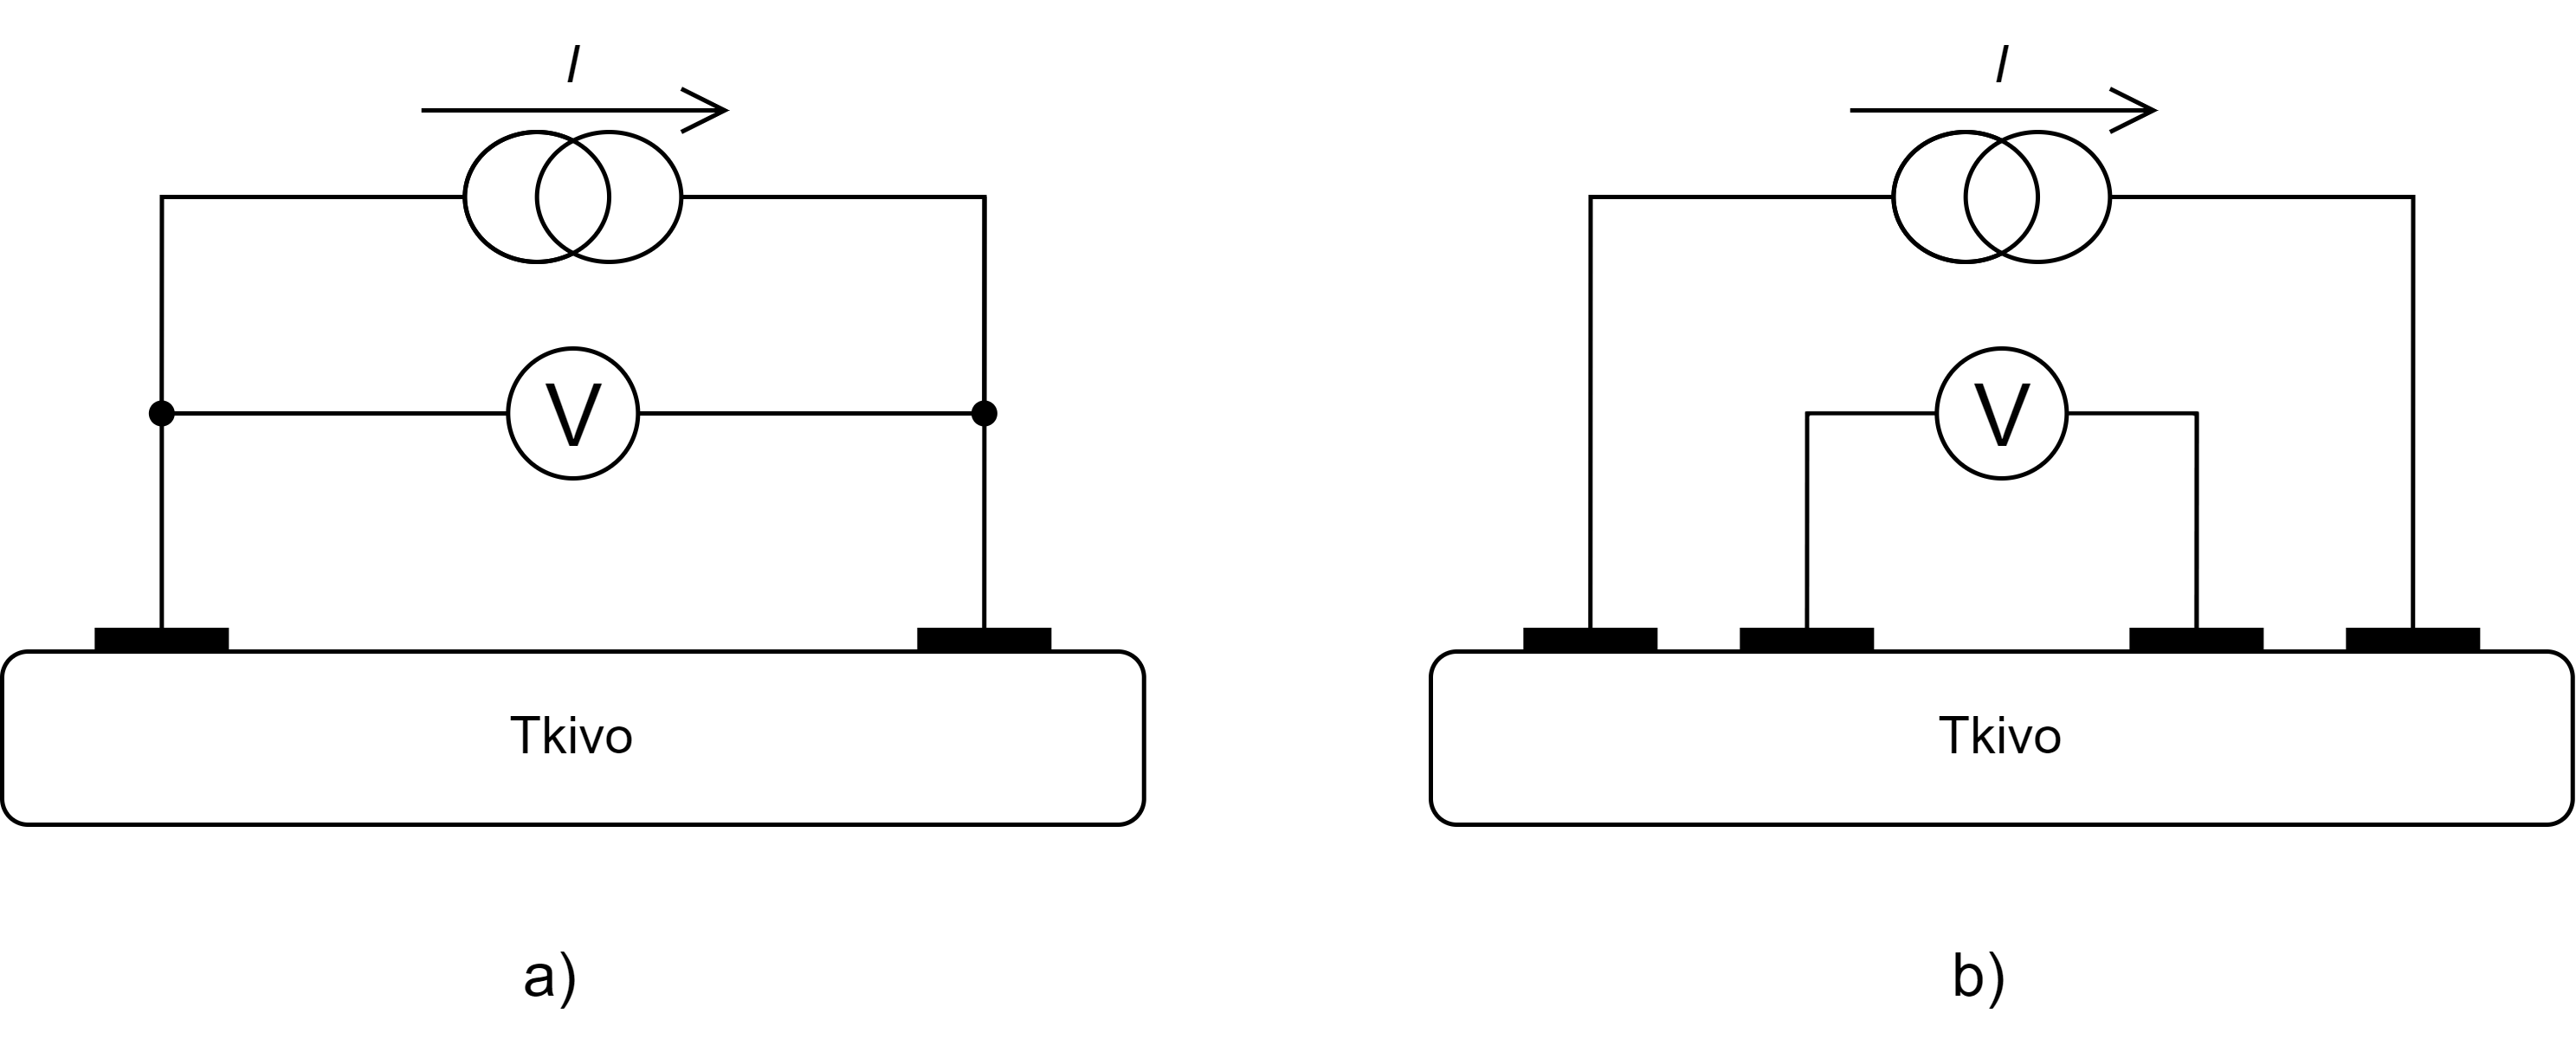
\includegraphics[width=0.8\textwidth]{Figures/dvo_vs_cetverozicno.png} 
    \caption{Dvožično (a) i četverožično (b) mjerenje bioimpedancije}
    \label{slk:cole_model}
\end{figure}

Važan dio mjernog sustava su i elektrode, koje kroz sučelje koža-elektroda omogućavaju protjecanje struje od mjernog sustava do tkiva. 
U ovom radu usporedit će se rezultati dobiveni s dvjema različitim vrstama elektroda: tradicionalnim metalnim elektrodama i tekstilnim elektrodama. 
Tekstilne elektrode izrađene su od tkanina impregniranih provodnim materijalima, najčešće srebrom. 
Njihova najveća prednost je udobnost i fleksibilnost te mogućnost integracije u odjeću.
Time ih pacijenti neometano mogu nositi tijekom svakodnevnih aktivnosti i dužeg perioda. 
Međutim, metalne elektrode su manje osjetljive na vanjske parametre kao što su temperatura i znojenje kože što daje pouzdanije rezultate mjerenja. 
\cite{Meding2021}

\begin{figure}[htb]
    \centering
    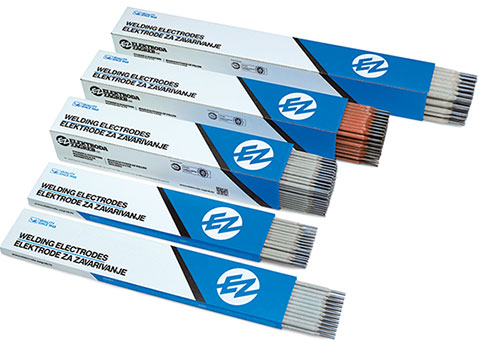
\includegraphics[width=0.6\textwidth]{Figures/electrode.jpg} 
    \caption{Tu će bit neka lijepa slika elektroda}
    \label{slk:elektrode}
\end{figure}

Sve opisane metode predstavljaju jednostavan i neinvazivan postupak mjerenja bioimpedancije. 
Važno je napomenuti kako izmjerena impedancija ovisi o brojim faktorima kao što su položaj tijela, hidracija, temperatura tijela i drugi 
što treba uzeti u obzir pri obradi rezultata mjerenja.

\section{Komercijalno dostupni uređaji za mjerenje bioimpedancije}

SFB7 ImpediMed

\end{document}